\documentclass[12pt]{article}

\usepackage{sbc-template}
\usepackage{graphicx,url}
\usepackage[portuguese]{babel}
\usepackage[utf8]{inputenc}
\usepackage[alf]{abntcite}
\usepackage{multirow}

\urlstyle{rm}

\sloppy

\title{Um Sistema de Apoio à Decisão para Auxílio na Mecânica Automotiva}

\author{José Lucas dos S. Borges{\inst1}}

\address{Departamento de Ciência da Computação -- Instituto de Matemática\\
    Universidade Federal da Bahia (UFBA)\\
    Rua Barão de Jeremoabo, s/n - Ondina, Salvador - BA, 40170-115
\email{jlucas@dcc.ufba.br}
}

\begin{document}

\maketitle

\begin{abstract}
    This paper proposes a Decision Support System (DSS) in the format of an
    mobile application in the automotive mechanics area, and it is aimed for
    lay people in this subject. Here are mentioned and discussed the variables
    used in the application, the types of Information System (IS) and DSS in
    which it fits, the main algorithms used and a brief system modelling, with
    some screen prototypes.
\end{abstract}

\begin{resumo}
    Este artigo propõe um Sistema de Apoio à Decisão (SAD) no formato de um
    aplicativo para celulares na área de mecânica automotiva para pessoas leigas
    no assunto. Aqui são apresentados e discutidos as variáveis utilizadas no
    aplicativo, os tipos de Sistema de Informação (SI) e SAD nos quais ele se
    enquadra, os principais algoritmos utilizados e uma breve modelagem do
    sistema, com alguns protótipos de tela.
\end{resumo}


\section{Introdução} \label{sec:introducao}

Mecânica automotiva é um assunto extremamente complexo. Cada um dos inúmeros
componentes do automóvel tem seu próprio ciclo de vida e devem ser revisados
e trocados em seu próprio tempo. Além disso, certas condições de uso podem
diminuir a vida útil de algumas peças, tornando mais frequente a necessidade
de revisão.

A falta de conhecimento destes fatos pode levar ao dono de um automóvel
negligenciar as manutenções no tempo correto, causando desde transtornos
que poderiam ser facilmente evitados a acidentes ocasionados por falhas
mecânicas.

O uso de um aplicativo para celular pode ser uma grande ajuda na decisão de
quando é necessário a revisão e troca de peças, alertando o usuário
visualmente quando alguma manutenção está próxima.

% \section{Referencial Teórico} \label{sec:referencialteorico}
% Esta seção aborda os principais fundamentos teóricos envolvidos na notificação
% oportuna de motoristas, tema central deste trabalho. Aqui são discutidos os
% conceitos de SI e SAD e os principais fatores que influenciam na manutenção
% automotiva.

\section{Manutenção Automotiva} \label{sec:manutencao}
Para descobrir quais são os principais fatores que influenciam na frequência de
manutenção de automóveis, foi feita uma busca nos manuais dos carros mais vendidos
no Brasil em 2016 que, segundo a Federação Nacional da Distribuição de Veículos
Automotores - Fenabrave - foram o Hyundai HB20, Chevrolet Onix e Ford Ka Hatch
\cite{fenabrave}.

Todos os manuais pesquisados citam três fatores importantes que influenciam na
frequência de manutenção de peças veiculares: a quilometragem do veículo, o
tempo desde sua última revisão e suas condições de uso \cite{manualhyundai,
manualonix, manualka}. De acordo com os manuais, a severidade das condições de
uso de um veículo é definida pelos seguintes fatores:

\begin{itemize}
  \item Funcionamento constante em tráfego urbano lento com paradas e partidas
  excessivas.
  \item Serviços de táxi e similares.
  \item Viagens frequentes de curta distância, sem que o motor alcance a
  temperatura de funcionamento normal.
  \item Viagens longas em estradas de terra e/ou areia (estradas irregulares,
  com areia ou lama excessiva).
  \item Funcionamento prolongado em marcha lenta.
  \item Quando o veículo permanece, com frequência, parado por mais de dois
  dias.
\end{itemize}

Quando há uma ou mais condições severas presentes no uso de um veículo, a
manutenção nas peças deve ser feita com mais frequência, geralmente na metade do
tempo da troca normal.

Para que a aplicação proposta detecte o momento certo para indicar ao usuário a
necessidade de se fazer manutenção, são utilizados algoritmos de árvore de
decisão e polinomiais.

\section{Sistemas de Informação e Sistemas de Apoio à Decisão} \label{sec:sisad}
Segundo \citeonline{guimaraes2004sistema}, Sistemas de Informação podem ser definidos
como todo conjunto de dados e informações que são organizados de forma
integrada, com o objetivo de atender à demanda e antecipar as necessidades dos
usuários.

Segundo \citeonline{falsarella2004sistemas} os Sistemas de Informação podem ser
separados em cinco categorias:

\begin{itemize}
    \item Sistemas Transacionais
    \item Sistemas Gerenciais
    \item Sistemas Executivos
    \item Sistemas Especialistas
    \item Sistemas de Apoio à Decisão
\end{itemize}

Os Sistemas de Apoio à Decisão, como definidos por \citeonline{o2001sistemas},
são sistemas de informação computadorizados que fornecem aos gerentes apoio
interativo de informações durante o processo de tomada de decisão.

Bonczek, Holsapple e Whinston citados por \citeonline{neto2000modelo}, dizem que
o SAD tem seu foco no gerenciamento com ênfase na flexibilidade e capacidade de
fornecer respostas rápidas, podendo ser iniciado e controlado pelo responsável
da tomada de decisões. Seus objetivos gerais são melhorar a eficácia, ou
qualidade, da decisão e eficiência do processo de tomada de decisão em nível de
planejamento e gerência.

\citeonline{kenneth2011sistemas} discorrem sobre os componentes de um SAD. Eles
citam que seus principais componentes são um banco de dados, um software de
sistema e uma interface de usuário.

O banco de dados SAD é uma coletânea de dados correntes ou históricos
proveniente de uma série de aplicações ou grupos. Pode ser, por exemplo, um
pequeno banco de dados dentro de um computador com um subconjunto de dados
carregados e possivelmente combinados com dados externos
\cite{kenneth2011sistemas}.

Um software de sistema SAD contém as ferramentas de software empregadas para
análise de dados. Pode conter várias ferramentas diferentes ou um conjunto de
modelos matemáticos e analíticos que pode ser disponibilizado para o usuário do
SAD \cite{kenneth2011sistemas}.

\citeonline{alter1980decision} classifica os SAD em sete tipos distintos,
baseados em suas operações:

\begin{itemize}
  \item Sistemas de desenho de arquivos;
  \item Sistemas de análise de dados;
  \item Sistemas de análise de informações;
  \item Modelos de contas;
  \item Modelos de representação;
  \item Modelos de otimização;
  \item Modelos de sugestão;
\end{itemize}

O presente trabalho propõe um Sistema de Apoio à Decisão que auxilia o usuário
a tomar decisões relacionadas à manutenção mecânica do seu carro.

\section{Variáveis do Sistema e Algoritmos Utilizados} \label{sec:algoritmos}
O Meu Possante tem o objetivo de auxiliar pessoas a manterem a manutenção do seu
veículo em dia. Com base no referencial teórico pesquisado, as variáveis
escolhidas para este sistema foram as seguintes:

\begin{table}[h]
\centering
\resizebox{\textwidth}{!}{
\begin{tabular}{|c|c|c|}
\hline
\textbf{Variável}               & \textbf{Descrição}                                                                                  & \textbf{Referência}                                                                                     \\ \hline
Quilometragem do veículo        & \begin{tabular}[c]{@{}c@{}}Quantidade (em KM) rodados\\ no total pelo veículo\end{tabular}          & \multirow{3}{*}{\begin{tabular}[c]{@{}c@{}}\\HYUNDAI, 2017;\\ CHEVROLET, 2017;\\ FORD, 2017\end{tabular}} \\ \cline{1-2}
Tempo desde à última manutenção & \begin{tabular}[c]{@{}c@{}}Data em que foi feita a\\ última revisão da peça em questão\end{tabular} &                                                                                                         \\ \cline{1-2}
Condições de uso do veículo     & \begin{tabular}[c]{@{}c@{}}Identifica se o uso do\\ veículo é severo ou não\end{tabular}            &                                                                                                         \\ \hline
\end{tabular}
}
\caption{Quadro de variáveis utilizadas no sistema}
\label{quadro-variaveis}
\end{table}

A informação de quilometragem será atualizada pelo usuário em intervalos
regulares e estes dados serão utilizados junto com um algoritmo polinomial
para predizer quando a quilometragem chegará em um determinado limiar. Essa
informação, juntamente com os valores das outras variáveis, serão utilizadas
para a montagem de uma árvore de decisão, que decidirá se é o momento certo de
notificar o usuário sobre a manutenção de um determinado item.

Nas próximas sessões são explicados com detalhes os algoritmos utilizados.

\subsection{Árvore de Decisão}\label{sec:arvorededecisao}
A árvore de decisão é uma estrutura utilizada principalmente na implementação de
sistemas especialistas e em problemas de classificação. As árvores de decisão
tomam como entrada uma situação descrita por um conjunto de atributos e retorna
uma decisão, que é o valor predito para o valor de entrada \cite{russell2003}.

\begin{figure}[h]
\centering
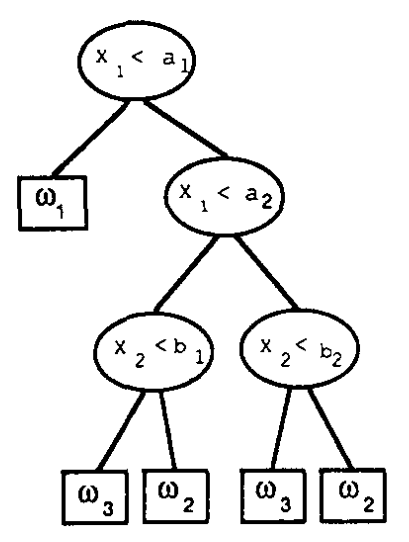
\includegraphics[width=0.3\textwidth]{arvorededecisao}
\caption{Exemplo de árvore de decisão \cite{safavian1991survey}}
\label{arvorededecisao}
\end{figure}

Uma árvore de decisão é composta de nós de decisão e nós-folha. Um nó de decisão
tem dois ou mais filhos, enquanto que um nó-folha representa uma classificação
ou decisão. O nó do topo da árvore, ou raiz corresponde ao elemento que melhor
classifica a informação em jogo. Árvores de decisão podem possuir tanto dados
categóricos como numéricos.

Árvores de decisão são atrativas por várias razões, entre elas a simplicidade,
eficiência, flexibilidade e performance \cite{safavian1991survey}.

\subsection{Algoritmo Polinomial}
Um algoritmo polinomial tenta construir uma função polinomial a partir de
valores já existentes. Com valores suficientes é possível construir uma curva
e predizer um determinado valor. A curva se torna mais precisa com quanto mais
valores forem informados.

%\section{Modelagem do Sistema} \label{sec:modelagem}

\bibliography{meu-possante}
%\bibliographystyle{sbc}

\end{document}
